\documentclass[11pt, a4paper]{article}
\usepackage[left=2cm,text={17cm, 24cm},top=3cm]{geometry}

\usepackage{times}
\usepackage[czech]{babel}
\usepackage[utf8]{inputenc}

%\usepackage[bottom]{footmisc}
\usepackage{hyperref}
\usepackage{multirow,multicol}
\usepackage[czech,linesnumbered,vlined,ruled,longend]{algorithm2e}
\usepackage{amsmath,mathtools}
\usepackage{graphicx}
\usepackage{pdflscape}


\begin{document}

\begin{titlepage}
\thispagestyle{empty}

    \begin{center}

        {\Huge \textsc{Vysoké učení technické v~Brně \\[0.3em]}}

        {\huge \textsc{Fakulta informačních technologií}}

        \vspace{\stretch{0.382}}

        {\LARGE{Typografie a publikování\,--\,3. projekt \\[0.3em]} 
        \Huge{Tabulky a obrázky} }

        \vspace{\stretch{0.618}}

        {\Large \today \hfill Boris Hatala (xhatal02)}
    \end{center}

\end{titlepage}
\newpage

\section{Úvodní strana}
    Název práce umístněte do zlatého řezu a nezapomeňte uvést \uv{dnešní} (today) datum 
    a vaše jméno a příjmení.
\section{Tabulky}
    Pro sázení tabulek můžeme použít prostředí\, \verb|tabbing| \, nebo prostředí\, \verb|tabular|.
\subsection{Prostředí \texttt{tabbing}}
Při použití \, \verb|tabbing| \, vypadá tabulka následovně:
\begin{table}[h]
    \begin{tabular}{l l l}
        \textbf{Ovoce} & \textbf{Cena} & \textbf{Množství} \\
        Jablka & 25,90 & 3 kg \\
        Hrušky & 27,40 & 2,5 kg \\
        Vodní melouny & 35,-- & 1 kus
    \end{tabular}
\end{table}
\bigskip
\\
\noindent
Toto prostředí se dá také použít pro sázení algorsitmů, ovšem vhodnější je 
použít prostředí \verb|alogorithm| nebo \verb|algorithm2e| (viz sekce ~\ref{sekce3}).
\subsection{Prostředí \texttt{tabular}}
Další možností, jak vytvořit tabulku, je použít prostředí\, \verb|tabular|. Tabulky pak budou vypadat
takto \footnote{Kdyby byl problém s~\, \texttt{cline,} 
zkuste se podívat třeba sem: \urlstyle{same}\url{http://www.abclinuxu.cz/tex/poradna/show/325037}.}:

\bigskip
\begin{table}[h] \catcode`\-=12
    \centering
        \begin{tabular}{|c|c|c|}
            \hline
                &\multicolumn{2}{|c|}{\textbf{Cena}} \\
            \cline{2-3}   
                \textbf{Měna} & \textbf{nakup} & \textbf{prodej} \\
                \hline
                EUR & 22,705 & 25,242 \\
                GBP & 25,931 & 28,828 \\
                USD & 21,347 & 23,732 \\
            \hline
        \end{tabular} \caption{Tabulka kurzů k~dnešnímu dni} \label{tab1}
\end{table}
\bigskip
\begin{table}[h] \catcode`\-=12
    \centering
        \begin{tabular}{|c|c|} \hline
            A~& A~\\ \hline
            P & N \\ \hline
            O~& O~\\ \hline
            X & X \\ \hline
            N & P \\\hline
        \end{tabular}
        \begin{tabular}{|cc|c|c|c|c|} \hline
            \multicolumn{2}{|c}{\multirow{2}{*}{$A \wedge B$}} & \multicolumn{4}{|c|}{$B$} \\ \cline{3-6}
             & & \textbf{P} & \textbf{O} & \textbf{X} & \textbf{N} \\ \hline
             \multicolumn{1}{|c|}{\multirow{4}{*}{$A$}} & \textbf{P} & P & O~& X & N \\ \cline{2-6}
             \multicolumn{1}{|c|}{} & \textbf{O} & O~& O~& N & N \\ \cline{2-6}
             \multicolumn{1}{|c|}{} & \textbf{X} & X & N & X & N \\ \cline{2-6}
             \multicolumn{1}{|c|}{} & \textbf{N} & N & N & N & N \\ \cline{2-6} \hline
        \end{tabular}
        \begin{tabular}{|cc|c|c|c|c|} \hline
            \multicolumn{2}{|c}{\multirow{2}{*}{$A \vee B$}} & \multicolumn{4}{|c|}{$B$} \\ \cline{3-6}
             & & \textbf{P} & \textbf{O} & \textbf{X} & \textbf{N} \\ \hline
             \multicolumn{1}{|c|}{\multirow{4}{*}{$A$}} & \textbf{P} & P & P & P & P \\ \cline{2-6}
             \multicolumn{1}{|c|}{} & \textbf{O} & P & O~& P & O~\\ \cline{2-6}
             \multicolumn{1}{|c|}{} & \textbf{X} & P & P & X & X \\ \cline{2-6}
             \multicolumn{1}{|c|}{} & \textbf{N} & P & O~& X & N \\ \cline{2-6} \hline
        \end{tabular}
        \begin{tabular}{|cc|c|c|c|c|} \hline
            \multicolumn{2}{|c}{\multirow{2}{*}{$A \to  B$}} & \multicolumn{4}{|c|}{$B$} \\ \cline{3-6}
             & & \textbf{P} & \textbf{O} & \textbf{X} & \textbf{N} \\ \hline
             \multicolumn{1}{|c|}{\multirow{4}{*}{$A$}} & \textbf{P} & P & O~& X & N \\ \cline{2-6}
             \multicolumn{1}{|c|}{} & \textbf{O} & P & O~& P & O~\\ \cline{2-6}
             \multicolumn{1}{|c|}{} & \textbf{X} & P & P & X & X \\ \cline{2-6}
             \multicolumn{1}{|c|}{} & \textbf{N} & P & P & P & P \\ \cline{2-6} \hline
        \end{tabular} \caption{Protože Kleeneho trojhodnotová logika už je \uv{zastaralá}, 
        uvádíme si zde příklad čtyřhodnotové logiky} \label{tab2}
\end{table}
\bigskip
\pagebreak

\section{Algoritmy}\label{sekce3}

Pokud budeme chtít vysázet algoritmus, můžeme použít prostředí 
\, \verb|algorithm|\footnote{Pro nápovědu, jak zacházet s~prostředím\, \texttt{algorithm,} \, můžeme zkusit tuhle stránku: \\\urlstyle{same}\url{http://ftp.cstug.cz/pub/tex/CTAN/macros/latex/contrib/algorithms/algorithms.pdf}.} \, 
nebo \, \verb|algorithm2e|\footnote{Pro \, \texttt{algorithm2e} \, zase tuhle: \urlstyle{same}\url{http://ftp.cstug.cz/pub/tex/CTAN/macros/latex/contrib/algorithm2e/doc/algorithm2e.pdf}.} \,. Příklad použití prostředí \, \verb|algorithm2e| \, viz Algoritmus \ref{alg1}.

\begin{algorithm}[h]\label{alg1}
    \SetAlgoNoLine
    \DontPrintSemicolon

    \SetNlSty{}{}{:}
    \SetAlgoNlRelativeSize{-1}
    \SetNlSkip{-1.2em}

    \caption{\textsc{FastSLAM}}

    \KwIn{\,$(X_{t-1}, u_t, z_t)$}
    \KwOut{\,$X_t$}

    \Indp \Indpp
    \BlankLine
    $\overline{X_t} = X_t = 0$\;
    \For{$k = 1$ \textup{to} $M$}{
        \Indpp 
        $x_t^{[k]} = sample\_motion\_model (u_t, x_{t-1}0^{[k]})$ \;
        $\omega_t^{[k]} = measurement\_model(z_t,x_t^{[k]},m_{t-1}) $\;
        $m t^{[k]} = updated\_occupancy\_grid(z_t, x_t^{[k]},m_{t-1}^{[k]}) $\;
        $\overline{X_t} = \overline{X_t} +\langle x_x^{[m]}, \omega_t^{[m]} \rangle$\;
    }
    \For{$k = 1$ \textup{to} $M$}{
        \Indpp
        draw $i$ with probability $\approx \omega_t^{[i]}$\;
        add $\langle x_x^{[k]}, m_t^{[k]} \rangle $ to $X_t$\;
    }
    \Return{$X_t$}
\end{algorithm}

\section{Obrázky}
Do našich článků můžeme samozřejmě vkládat obrázky. 
Pokud je obrázkem fotografie, můžeme klidně použít bitmapový
 soubor. Pokud by to ale mělo být nějaké schéma nebo něco 
 podobného, je dobrým zvykem takovýto obrázek vytvořit vektorově.
    
\begin{figure}[h] 
    \centering
    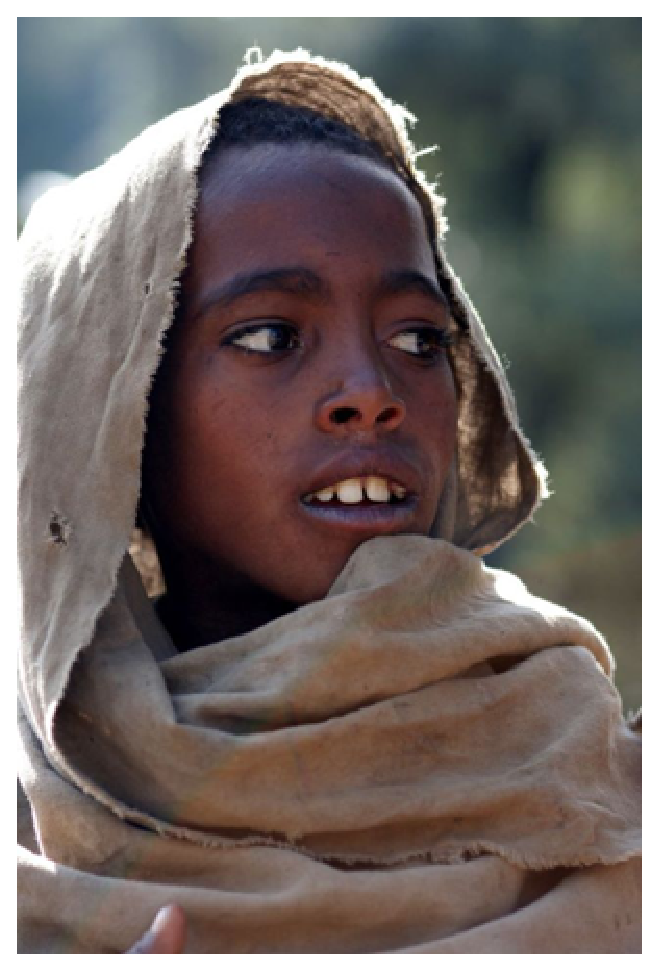
\includegraphics[scale=.4]{etiopan.eps}
    \reflectbox{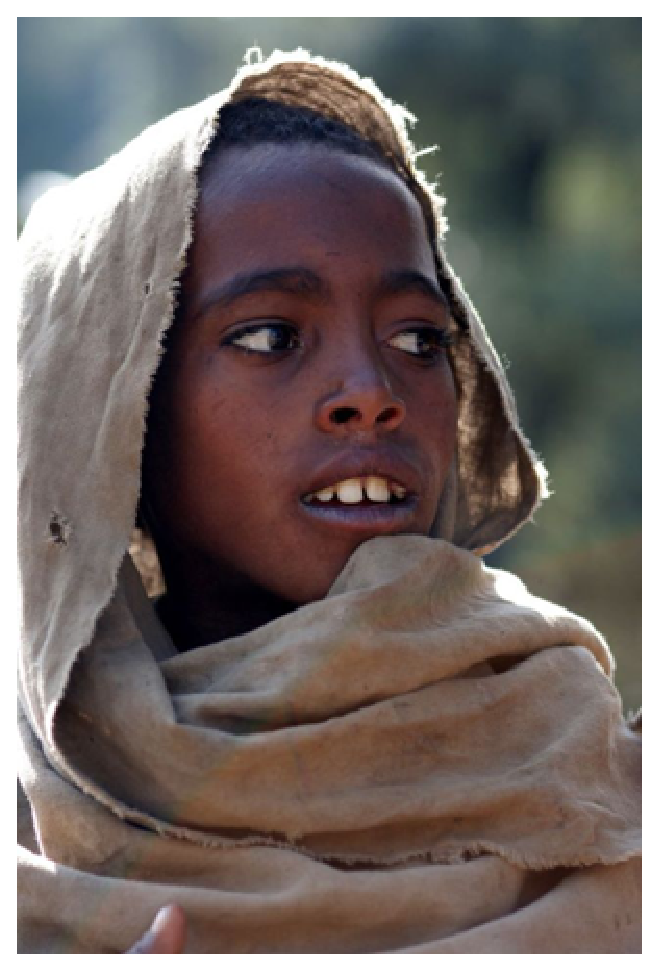
\includegraphics[scale=.4]{etiopan.eps}}
    \caption{Malý Etiopánek a jeho bratříček} \label{obr1}
\end{figure}
\pagebreak
Rozdíl mezi vektorovým \dots
\begin{figure}[h] 
    \centering
    
\includegraphics[scale=.4]{oniisan.eps}
    \caption{Vektorový obrázek}\label{obr2}
\end{figure}
\bigskip

\noindent
\dots a bitmapovým obrázkem
\begin{figure}[h] 
    \centering
    
\includegraphics[scale=.6]{oniisan2.eps}
    \caption{Bitmapový obrázek}\label{obr3}
\end{figure} 
\bigskip 
\\
se projeví například při zvětšení.\par
Odkazy (nejen ty) na obrázky \ref{obr1}, \ref{obr2} a \ref{obr3}, na tabulky \ref{tab1} a \ref{tab2} a 
také na algoritmus \ref{alg1} jsou udělány pomocí křížových odkazů. 
Pak je ovšem potřeba zdrojový soubor přeložit dvakrát.\par
Vektorové obrázky lze vytvořit i přímo v~\LaTeX u, 
například pomocí prostředí \, \verb|picture.| \,

\newpage
\setlength{\unitlength}{1cm}
\begin{landscape}
    \begin{figure}
    \begin{picture}(24,12)
        %frame
        \put(0,0){\line(0,1){12}}
        \put(24,0){\line(0,1){12}}
        \put(0,12){\line(1,0){24}}
        \put(0,0){\line(1,0){24}}

        %house outer line
        \put(8,1){\line(0,1){9}}
        \put(16,1){\line(0,1){9}}
        \put(8,1){\line(1,0){8}}
        \put(8,10){\line(1,0){8}}

        %windows
        \put(9,9){\line(1,0){2}}
        \put(9,7.5){\line(1,0){2}}
        \put(9,7.5){\line(0,1){1.5}}
        \put(11,7.5){\line(0,1){1.5}}
        \put(10.1,8.7){\line(-1,-1){0.8}}
        \put(10.3,8.4){\line(-1,-1){0.5}}

        \put(9,6){\line(1,0){2}}
        \put(9,4.5){\line(1,0){2}}
        \put(9,4.5){\line(0,1){1.5}}
        \put(11,4.5){\line(0,1){1.5}}
        \put(10.1,5.7){\line(-1,-1){0.8}}
        \put(10.3,5.4){\line(-1,-1){0.5}}

        \put(13,9){\line(1,0){2}}
        \put(13,7.5){\line(1,0){2}}
        \put(13,7.5){\line(0,1){1.5}}
        \put(15,7.5){\line(0,1){1.5}}
        \put(14.1,8.7){\line(-1,-1){0.8}}
        \put(14.3,8.4){\line(-1,-1){0.5}}

        \put(13,6){\line(1,0){2}}
        \put(13,4.5){\line(1,0){2}}
        \put(13,4.5){\line(0,1){1.5}}
        \put(15,4.5){\line(0,1){1.5}}
        \put(14.1,5.7){\line(-1,-1){0.8}}
        \put(14.3,5.4){\line(-1,-1){0.5}}

        %house door
        \put(11.4,1){\line(0,1){2}}
        \put(12.6,1){\line(0,1){2}}
        \put(11.1,3){\line(1,0){1.8}}
        \put(12.3,1.9){\circle*{0.15}}

        %garage
        \put(16,4.5){\line(1,0){5}}
        \put(21,1){\line(0,1){3.5}}
            %door
        \put(17,1){\line(0,1){2.5}}
        \put(20,1){\line(0,1){2.5}}
        \put(17,3.5){\line(1,0){3}}
        \put(18.5,1.4){\circle*{0.15}}
            %roof
        \put(16,6.17){\line(3,-1){6.5}}
        \put(16.5,4.5){\line(0,1){1.5}}
        \put(17,4.5){\line(0,1){1.35}}
        \put(17.5,4.5){\line(0,1){1.2}}
        \put(18,4.5){\line(0,1){1.05}}
        \put(18.5,4.5){\line(0,1){0.85}}
        \put(19,4.5){\line(0,1){0.7}}
        \put(19.5,4.5){\line(0,1){0.55}}
        \put(20,4.5){\line(0,1){0.35}}

        %tree
        \put(4.5,1){\line(0,1){2}}
        \put(5,1){\line(0,1){2}}
        \put(3.5,3){\line(1,0){2.5}}
        \put(3.5,3){\line(1,4){1.25}}
        \put(6,3){\line(-1,4){1.25}}

        %sun
        \put(3,10){\circle{2}}

        %base
        \linethickness{2mm}
        \put(2,1){\line(1,0){20}}

    \end{picture}
    \caption{Vektorový obrázek moderního bydlení vhodného 
    pro 21. století. (Buďto vytvořte stejný obrázek, anebo nakreslete
    pomocí\, \texttt{picture}\, váš vlastní domov.)}
    \end{figure}
    
\end{landscape}
\end{document}  